\section{操作説明}
    \subsection{投稿範囲の設定}
    \begin{enumerate}
        \item 設定画面の\ttbox{なうぷれ設定}→\ttbox{詳細}を押下して展開してください。
            \begin{figure}[htbp]
                \begin{minipage}[b]{0.45\linewidth}
                    \centering
                    \fbox{
                        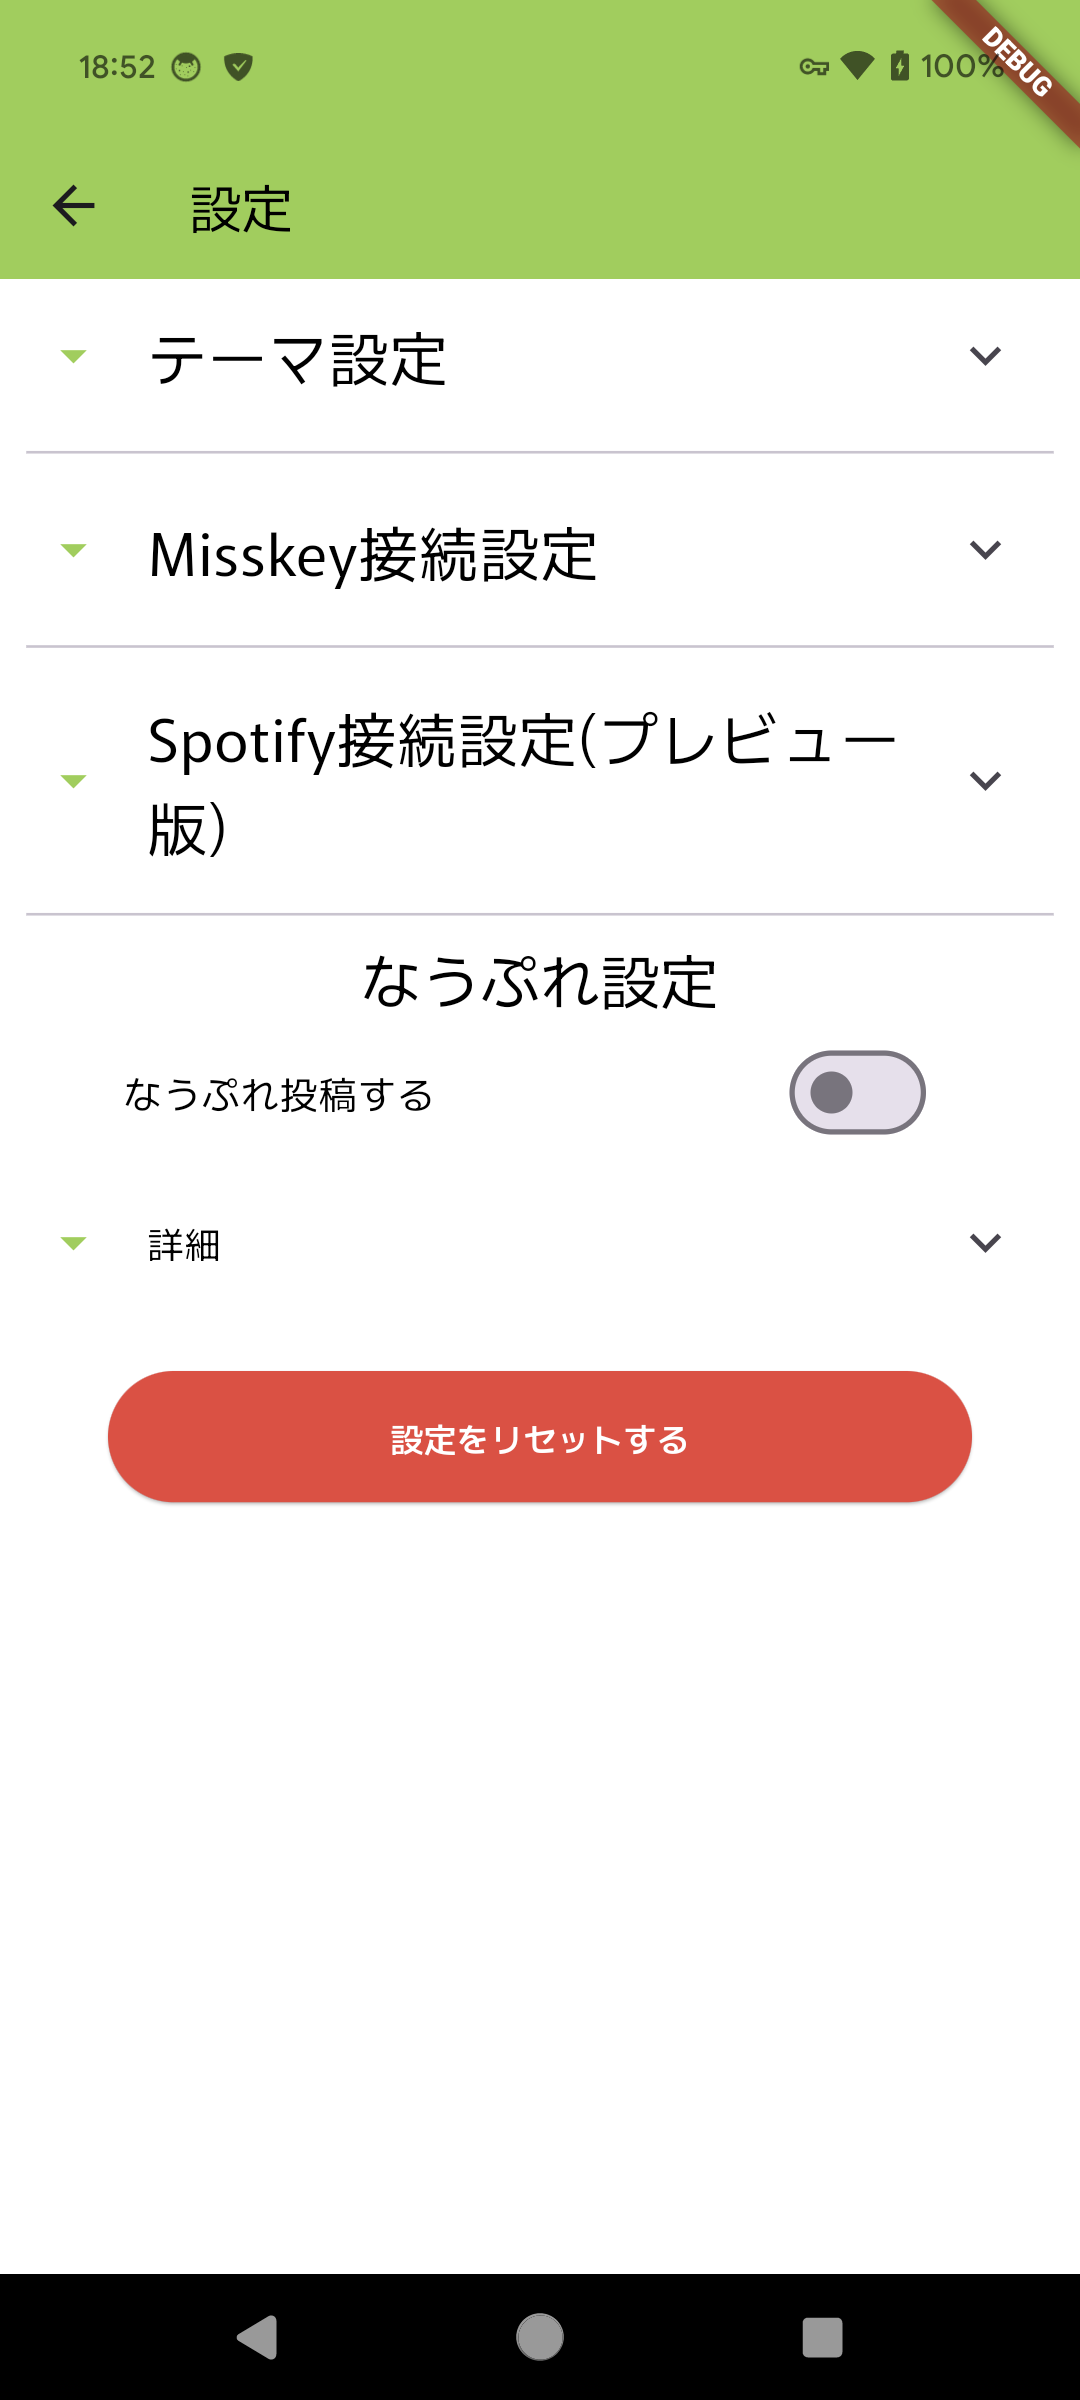
\includegraphics[width=5cm]{./pictures/guide1.png}
                    }
                    \caption{展開前}
                    \label{img:guide1}
                \end{minipage}
                \begin{minipage}[b]{0.45\linewidth}
                    \centering
                    \fbox{
                        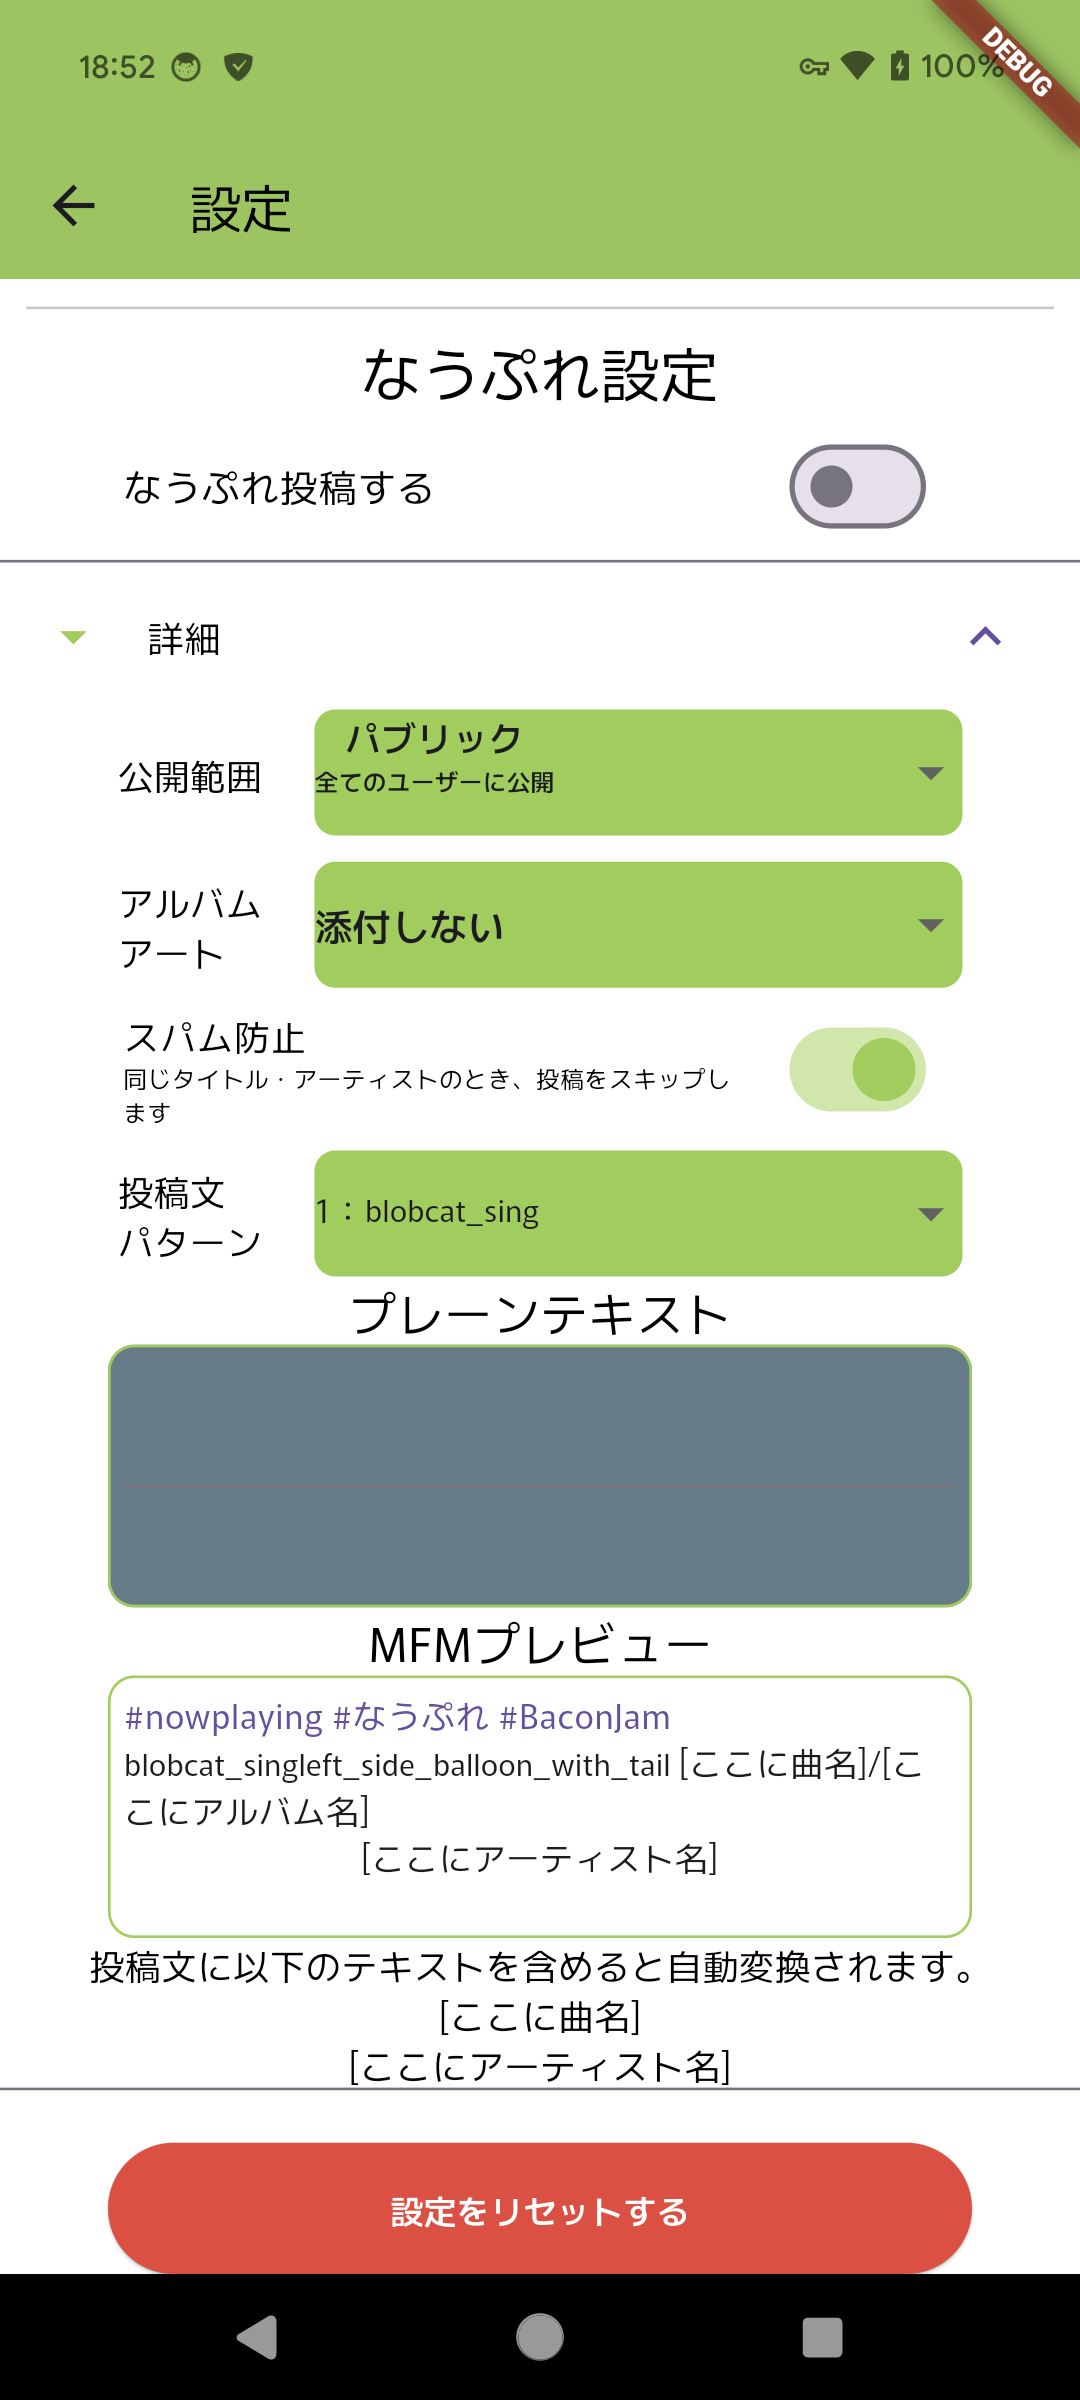
\includegraphics[width=5cm]{./pictures/guide2.png}
                    }
                    \caption{展開後}
                    \label{img:guide2}
                \end{minipage}
                \caption*{\mi なうぷれ設定の詳細(\currentVersion)}
            \end{figure}

        \newpage
        \item 公開範囲のドロップダウンで\ttbox{チャンネル}を選択して、\ttbox{チャンネルを選択}を押下してください。
            \begin{figure}[htbp]
                \begin{minipage}[b]{0.45\linewidth}
                    \centering
                    \fbox{
                        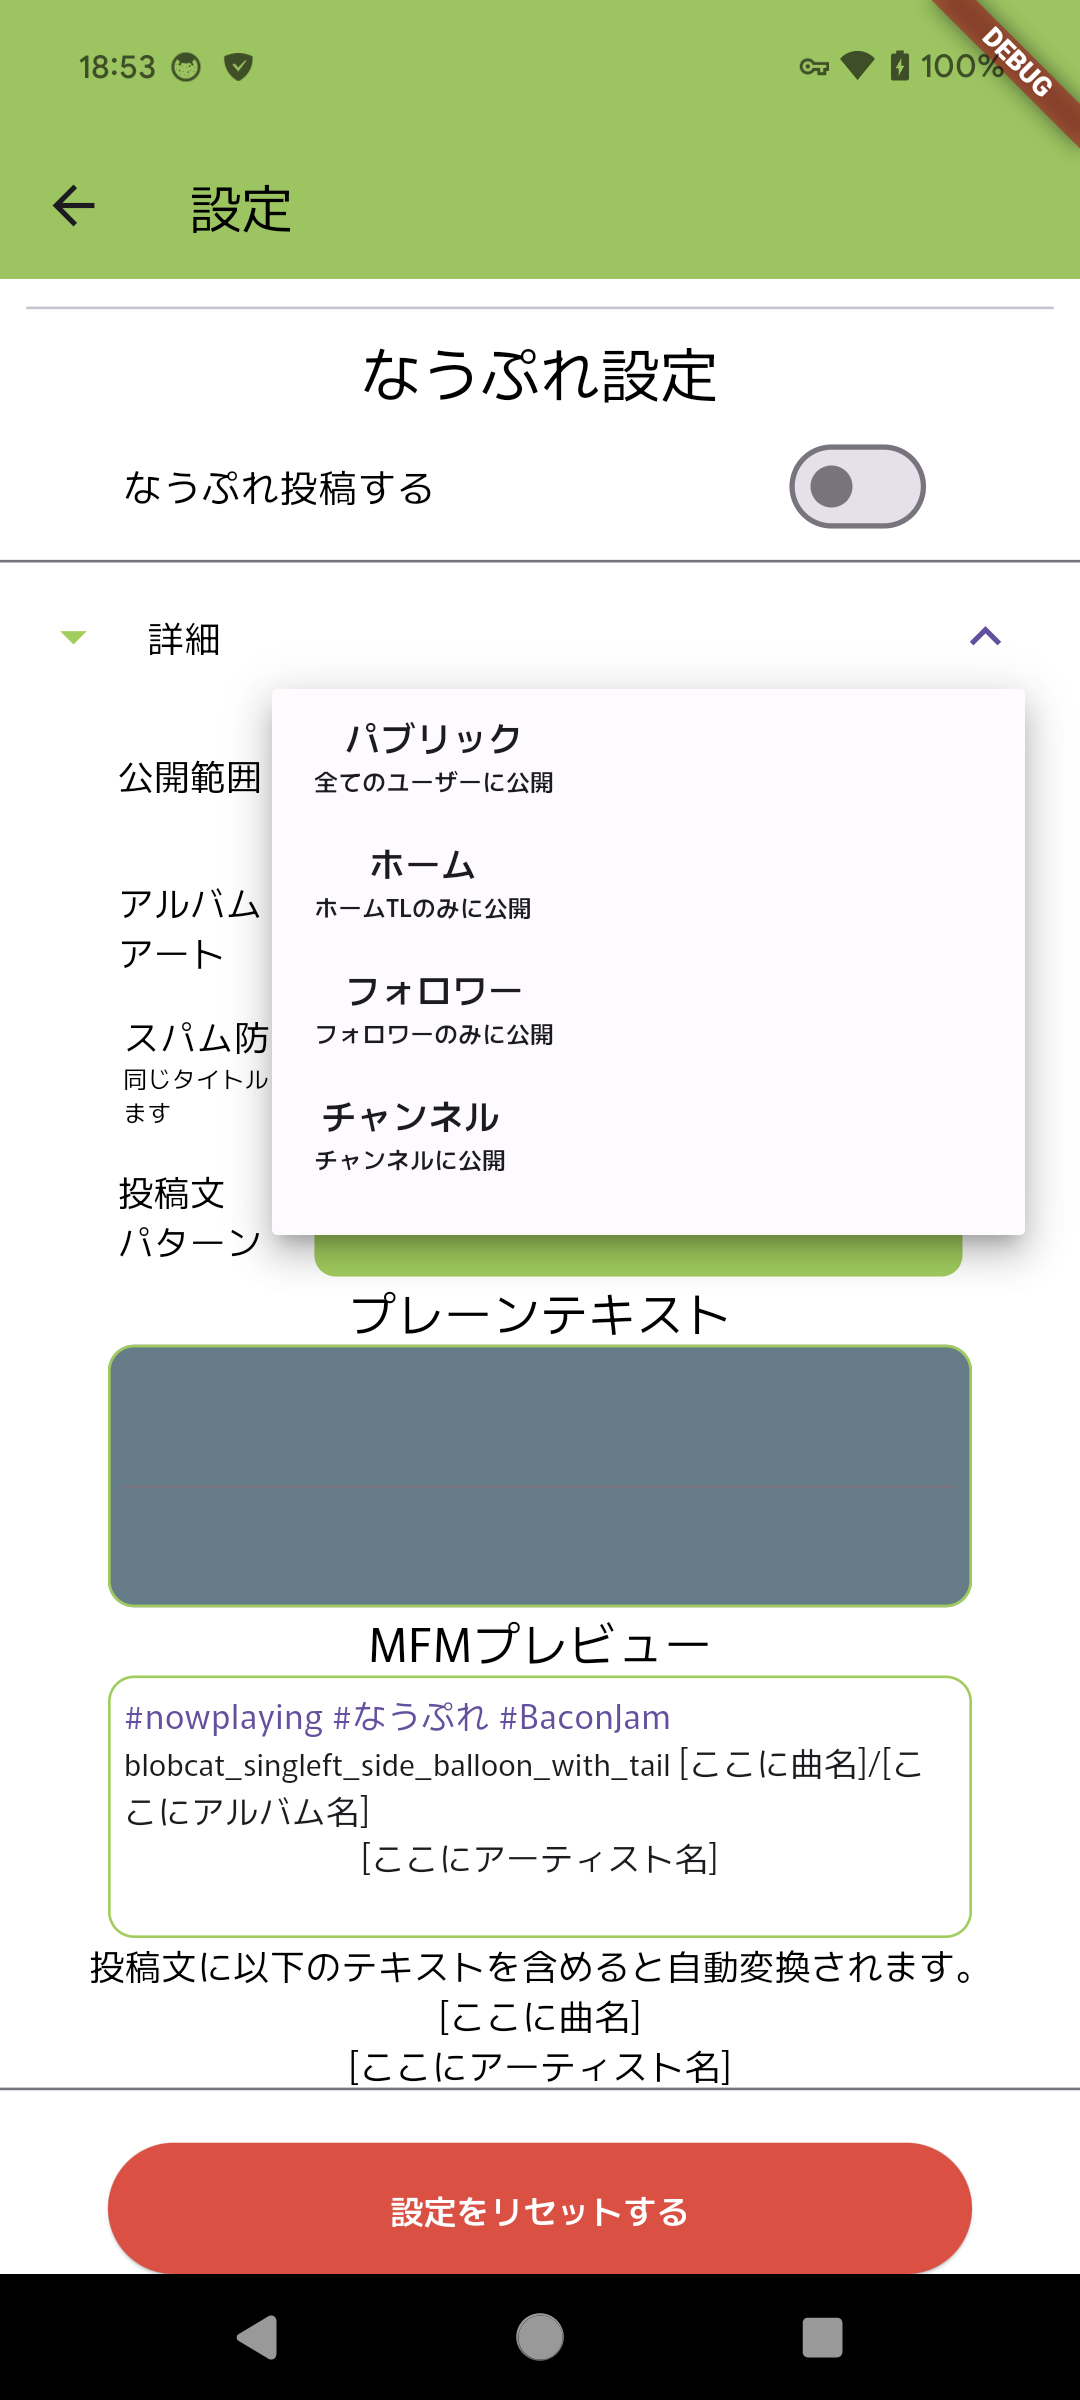
\includegraphics[width=5cm]{./pictures/guide3.png}
                    }
                    \caption{ドロップダウン一覧}
                    \label{img:guide3}
                \end{minipage}
                \begin{minipage}[b]{0.45\linewidth}
                    \centering
                    \fbox{
                        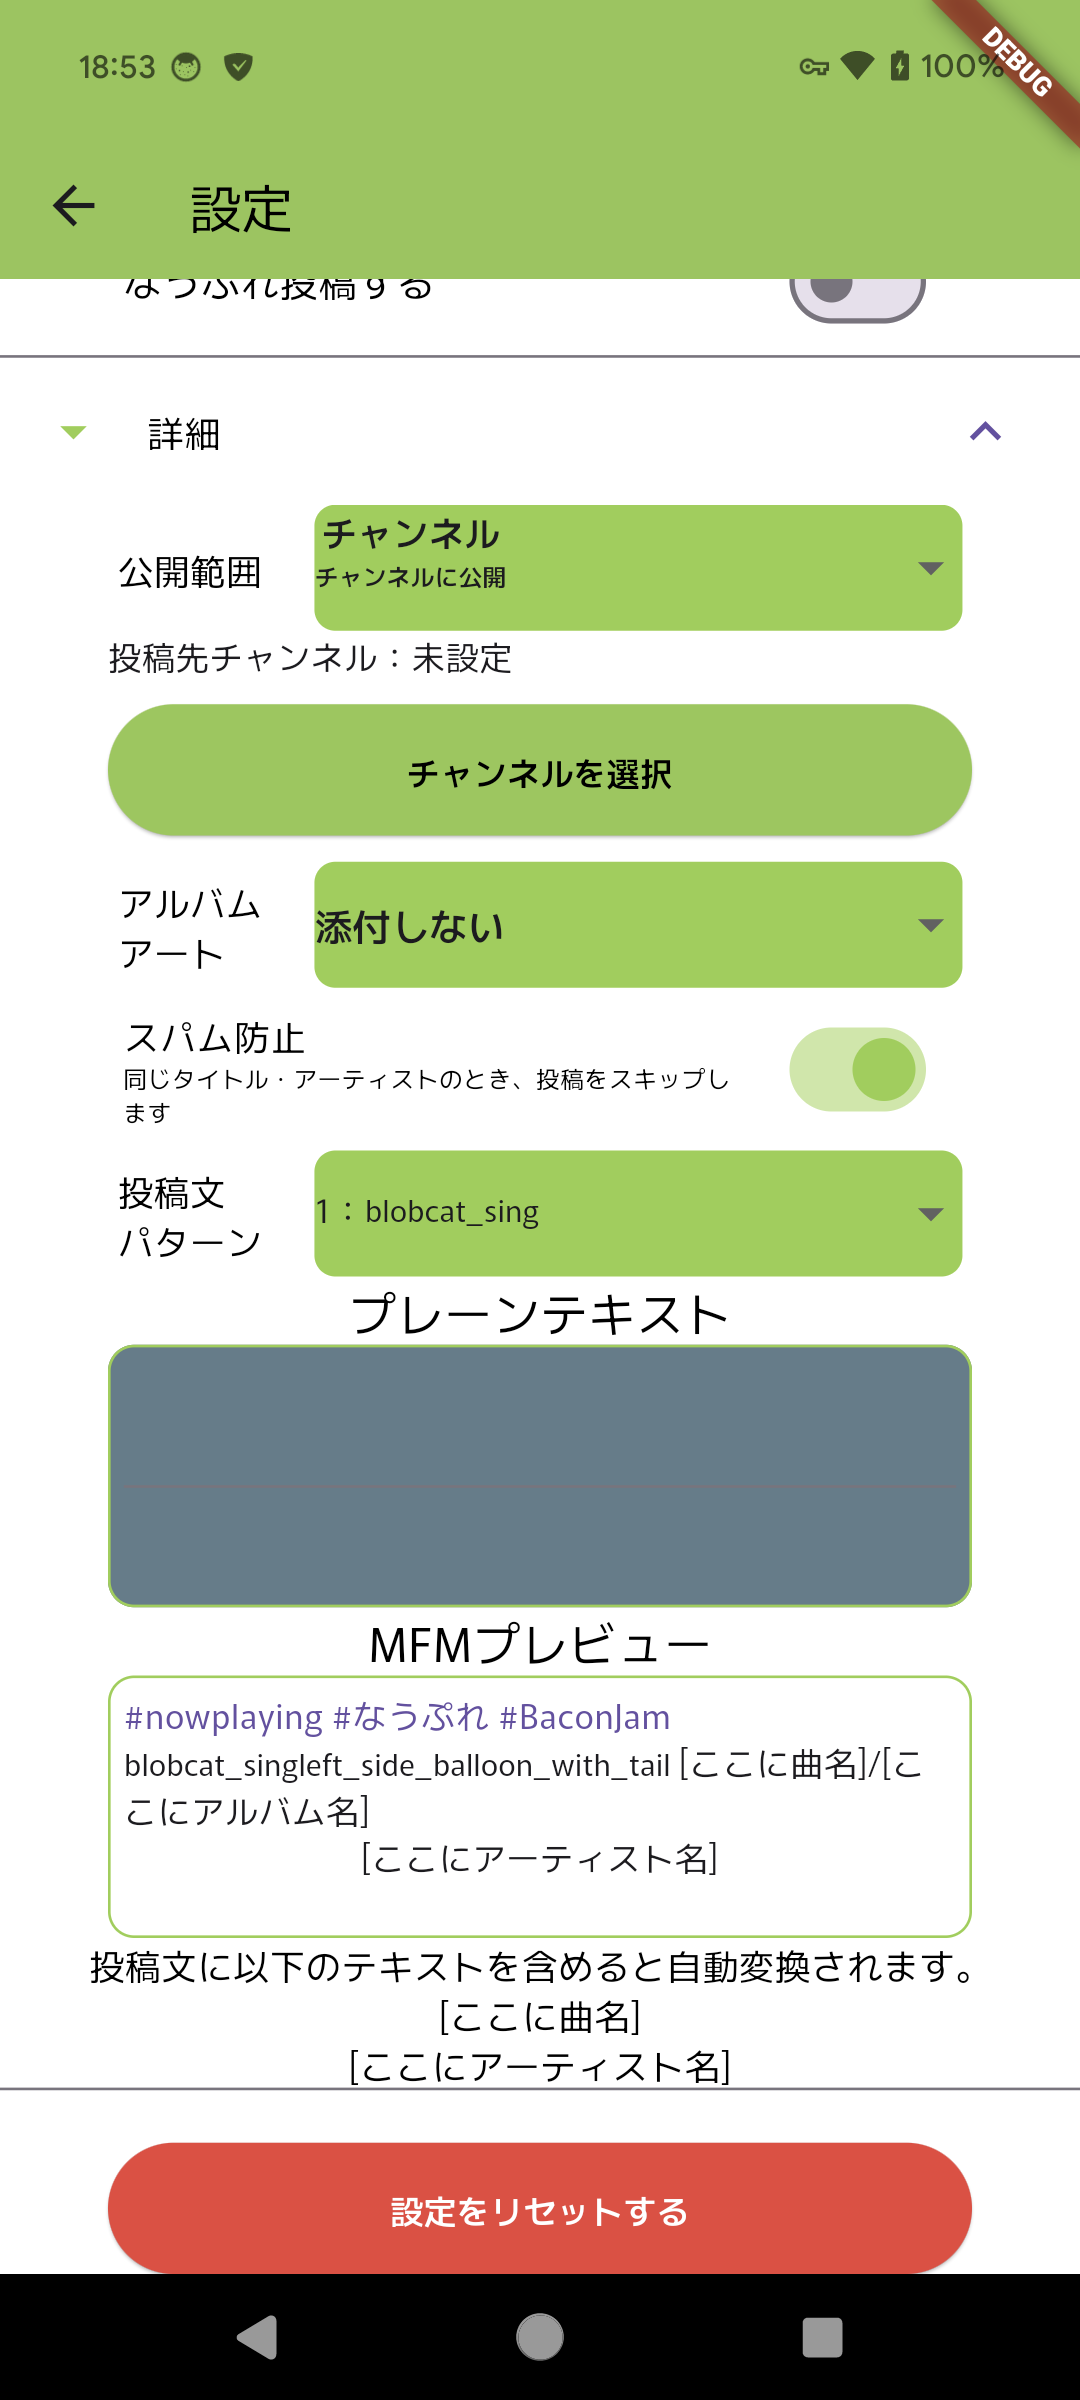
\includegraphics[width=5cm]{./pictures/guide4.png}
                    }
                    \caption{チャンネルを選択した場合}
                    \label{img:guide4}
                \end{minipage}
                \caption*{\mi 公開範囲の選択(\currentVersion)}
            \end{figure}

        \newpage
        \item チャンネル検索ページで、チャンネルの名称を入力して検索してください。
            \begin{figure}[htbp]
                \centering
                \fbox{
                    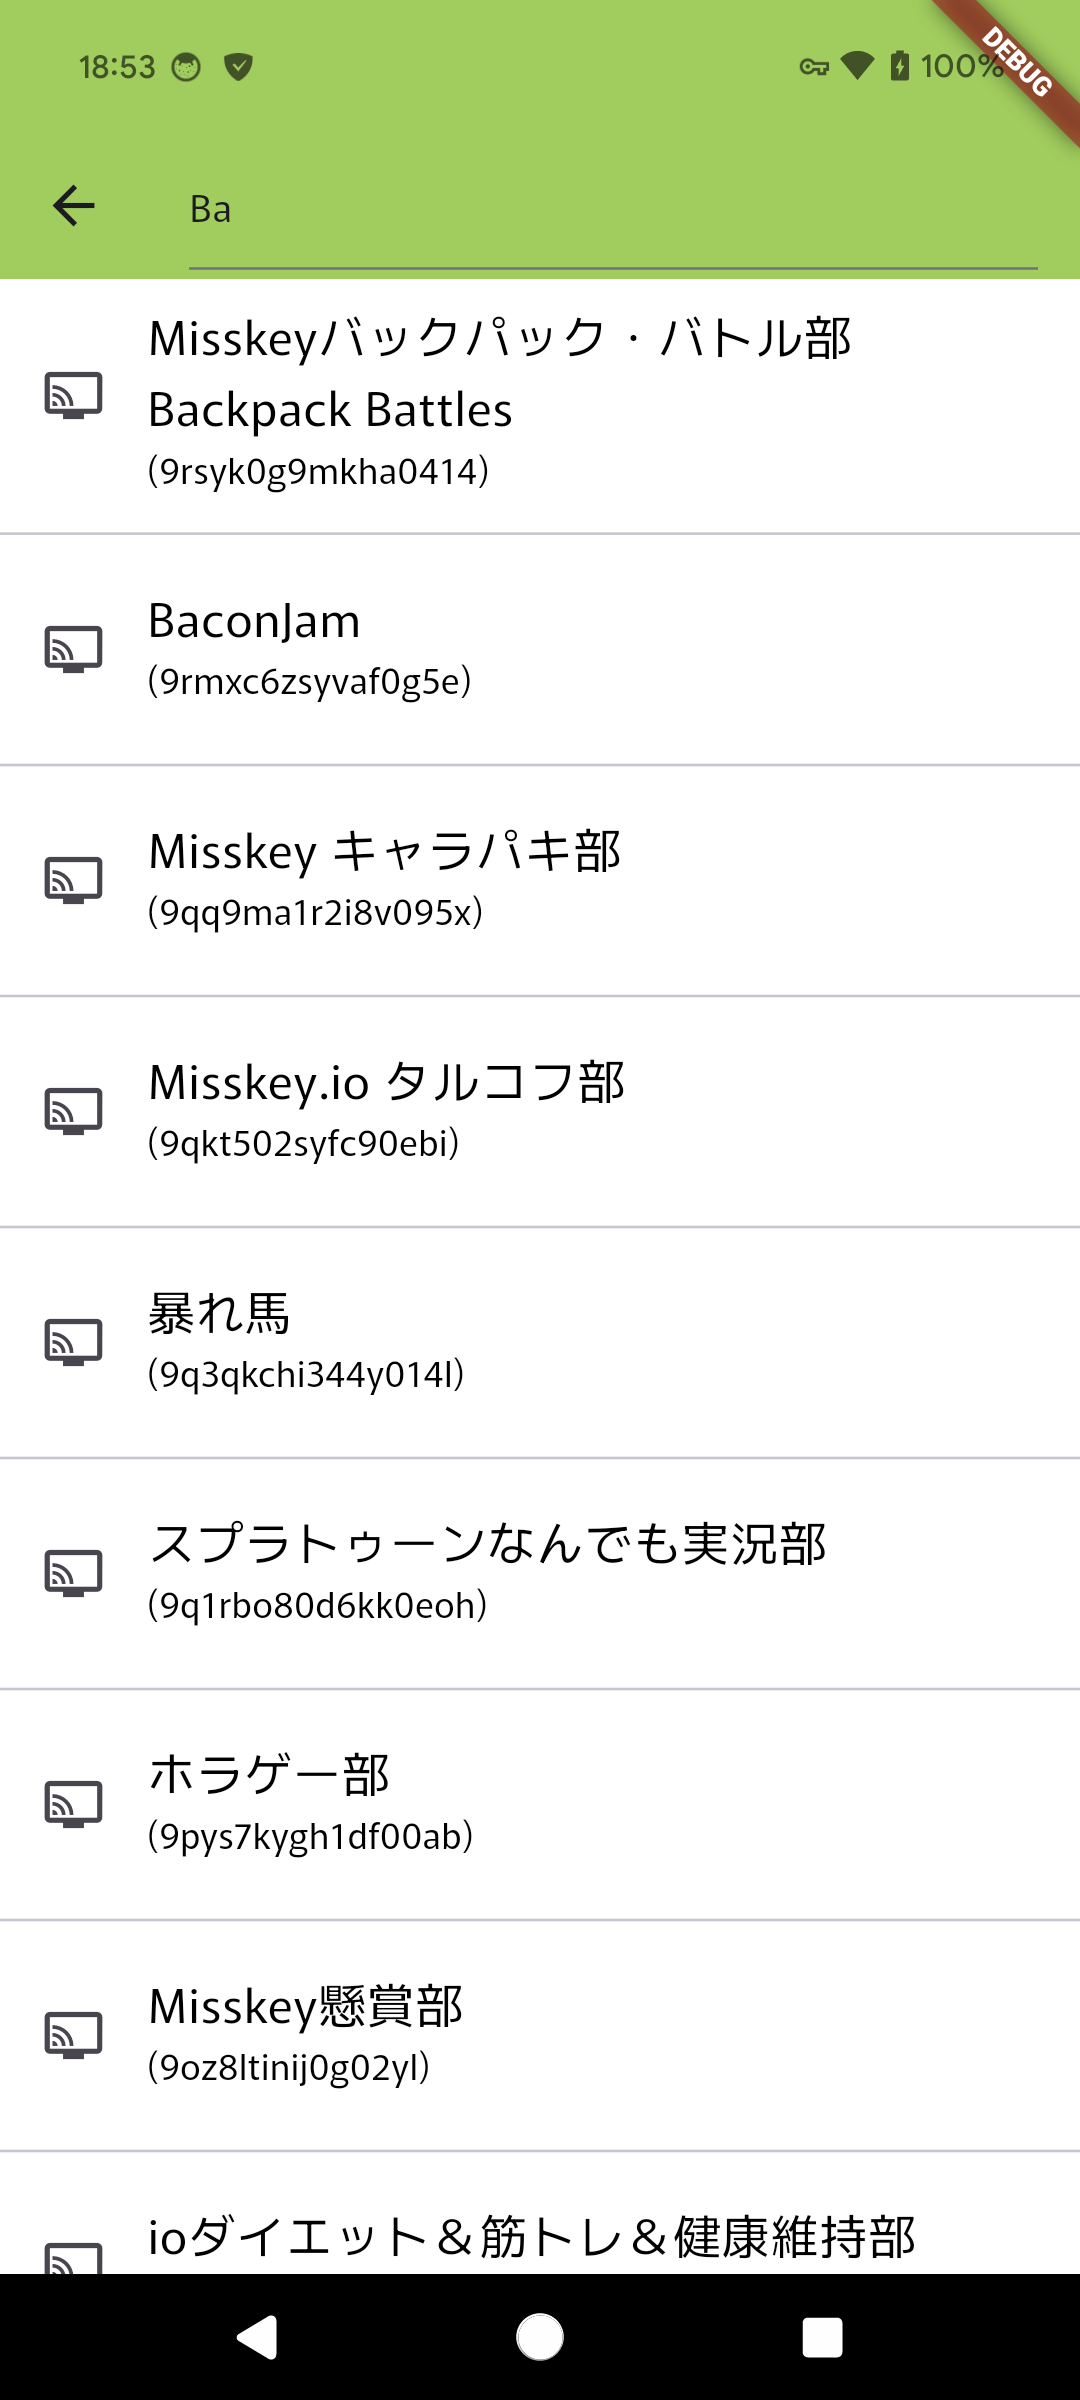
\includegraphics[width=5cm]{./pictures/guide5.png}
                }
                \caption{チャンネル検索ページ(\currentVersion)}
                \label{img:guide5}
            \end{figure}

        \newpage
        \item 投稿したいチャンネル名を押下すると、そのチャンネルを指定して設定画面に戻ります。
            \begin{figure}[htbp]
                \centering
                \fbox{
                    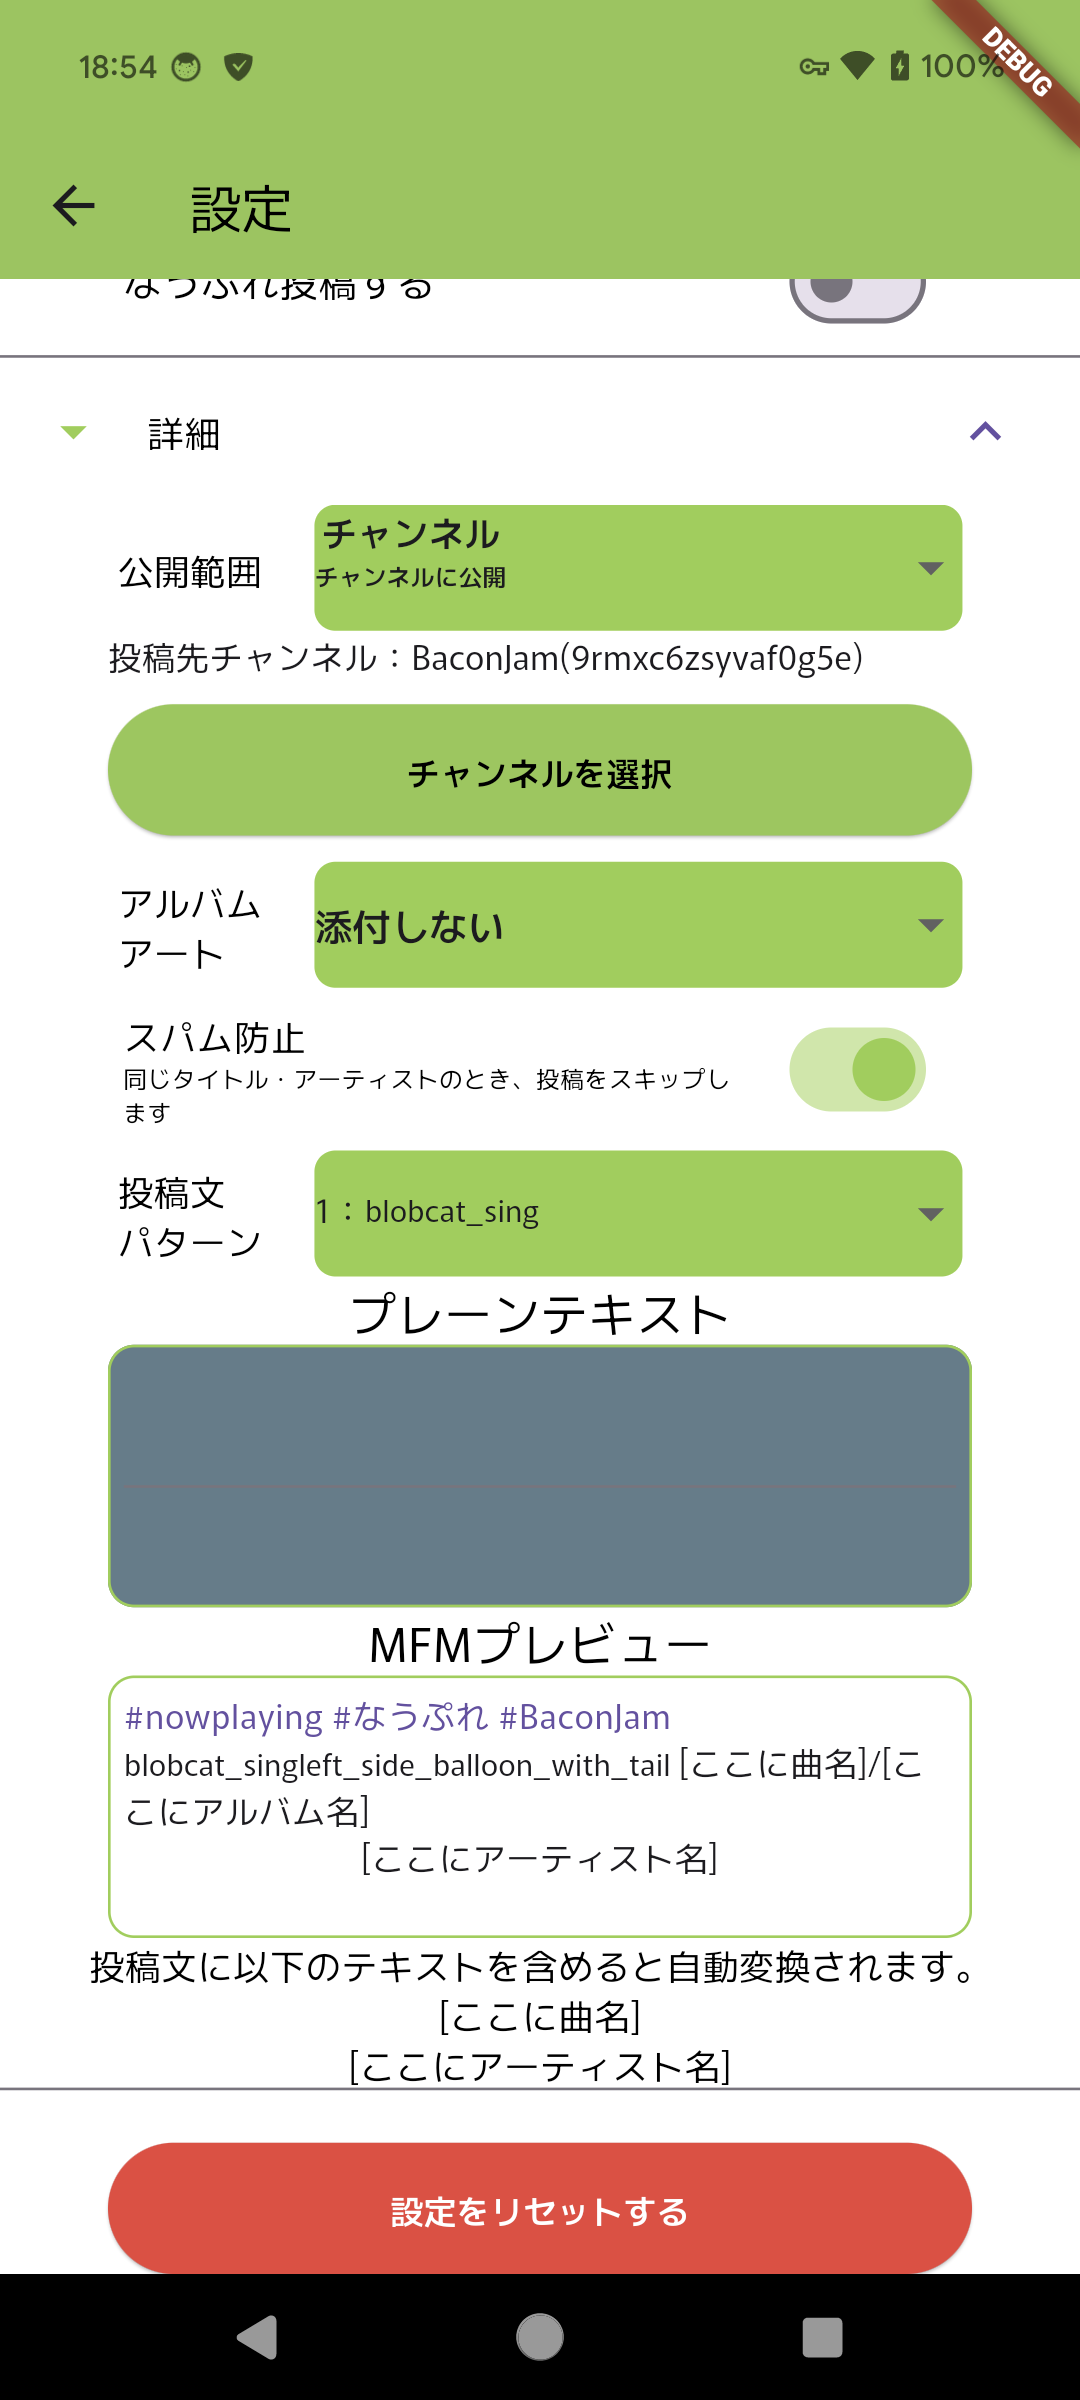
\includegraphics[width=5cm]{./pictures/guide6.png}
                }
                \caption{チャンネル指定後(\currentVersion)}
                \label{img:guide6}
            \end{figure}
    \end{enumerate}
